\documentclass{article}

% Essential packages
\usepackage{graphicx}   % For image handling
\usepackage{subcaption} % For multi images
\usepackage{caption}    % For proper captions
\usepackage{listings}   % For code listings
\usepackage{fontspec}   % For custom fonts
\usepackage{xcolor}     % For color support
\usepackage{tcolorbox}  % For code block boxes
\usepackage{etoolbox}   % For patching and command manipulation
\usepackage{titlesec}   % For section formatting
\usepackage{parskip}    % For customisable paragraph formating
\usepackage{comment}    % For being able to comment out sections
\usepackage{geometry}   % For managing page size and margins
\usepackage{hyperref}   % For embedding links, like URL's

\tcbuselibrary{listings, skins, breakable}  %Librarary to make code blocks multipage


%   ############################## Customisation ##############################

% Document metadata
\title{\fontsize{24}{36}\selectfont Programable Logic Circuts\\ %Edit title here \\ means new line
Lab 01} % Line 2 of title, its not subtitle, that is possible to, google it
\author{Sølve Kjelseth} %I nput your name
\date{\today} % Auto updates the date, untill you export it, replace with hardcoded date if you need

% Adjust the body text font size to 12pt without affecting section headings
\renewcommand{\normalsize}{\fontsize{12}{16}\selectfont}

% Adjust the paragraph spacing, either as indentation or/and line spaceing
\setlength{\parindent}{0pt}  % Remove indentation
\setlength{\parskip}{6pt}    % Add vertical space between paragraphs

% Customisation of fonts and colors
\setmainfont{Times New Roman}
\setmonofont{JetBrains Mono}
\definecolor{background}{RGB}{225, 219, 202}
\definecolor{darkAccent}{RGB}{140, 98, 64}
\definecolor{commentGreen}{RGB}{26, 159, 32}
\definecolor{keywordPurple}{RGB}{229, 24, 192}
\definecolor{keywordBlue}{RGB}{5, 142, 217}
\definecolor{portOrange}{RGB}{234, 72, 31}
\definecolor{darkGray}{RGB}{60, 60, 60}

%Link
\hypersetup{
    colorlinks=true,
    linkcolor=darkGray,    
    urlcolor=keywordBlue
    }

\urlstyle{same}


% Customisation of margins and paper size
\geometry{
 a4paper,
 left = 30mm,
 right = 30mm,
 top = 30mm,
 bottom = 30mm
 }

% Sections formatting and numbering

% Sets the font to monospace for section, subsection and subsubsection
% and sets the format to be numbers with . between and at the end
\renewcommand{\thesection}{\texttt{\arabic{section}.}}
\renewcommand{\thesubsection}{\texttt{\arabic{section}.\arabic{subsection}.}}
\renewcommand{\thesubsubsection}{\texttt{\arabic{section}.\arabic{subsection}.\arabic{subsubsection}.}}

\setcounter{section}{-1}  % Start section numbering from 0, delete this to start from 1

% Makes section monospace font and start each subsection from 0
\let\oldsection\section
\renewcommand{\section}[1]{%
  \oldsection{\texttt{#1}} % Make section title monospace
  \setcounter{subsection}{-1} % Makes subsection start from 0, delete this line to start from 1
  \setcounter{figure}{-1} % Makes figure numbers start from 0, delete this line to start from 1
}

% Makes subsection monospace font and start each subsubsection from 0
\let\oldsubsection\subsection
\renewcommand{\subsection}[1]{%
  \oldsubsection{\texttt{#1}}% Make subsection title monospace
  \setcounter{subsubsection}{-1}% Makes subsubsection start from 0, delete this line to start from 1
}

% Makes subsubsection monospace font
\let\oldsubsubsection\subsubsection
\renewcommand{\subsubsection}[1]{%
  \oldsubsubsection{\texttt{#1}}% Make subsubsection title monospace
}

% Makes every new section start on a new page, except for the first section, section 0
\pretocmd{\section}{%
  \ifnum\value{section}=-1 \else\clearpage\fi % Replace -1 with 0 if sections start at nr. 1
}{}{}

% Makes every figure be formated as section number.figure number
\renewcommand{\thefigure}{\arabic{section}.\arabic{figure}}

% Add keywords to be highlited in blue below. Note that all reserved
% keywords from VHDL is already in purple and should not be added here
% too as duplicates will cause issues. Therfore compile this document
% after pasting in code and only add non-highlited words to this list.
% Also, there is not a list for orange keywords, used for ports here.
\lstdefinelanguage{VHDL+}{
    language     = VHDL,
    morestring = [b]',
    morekeywords = [2]{
        IEEE,
        std_logic_1164, std_logic, std_logic_vector},
    morekeywords = [3]{
        SW, LEDR, KEY,
        HEX0, HEX1, HEX2, HEX3, HEX4, HEX5, HEX6},
    sensitive = false
}

% Makes Table of contents a subsection
\makeatletter
\renewcommand{\tableofcontents}{%
    \subsection{Table of Contents} % Numbered subsection named Table of contents
    \@starttoc{toc}%
}
\makeatother


% Makes Table of contents a subsection
\makeatletter
\renewcommand{\listoffigures}{%
    \subsection{List of Figures} % Numbered subsection named List of figures
    \@starttoc{lof}%
}
\makeatother


\newcommand{\introduction}[1][]{%
    \addtocontents{toc}{\protect\setcounter{tocdepth}{0}} % Temporarily hide from TOC
    \section{Introduction} % Numbered section named Introduction
    \ifx\relax#1\relax % Check if argument is empty
    \else
        #1 % Insert the optional text if provided
    \fi
    \tableofcontents % Generate TOC
    \clearpage
    \listoffigures % List of figures
    \addtocontents{toc}{\protect\setcounter{tocdepth}{2}} % Restore TOC depth
}


%   ############################## Advanced customisation ##############################

% Customisation of list style inside code block
\lstdefinestyle{VHDL}{
    language = VHDL+, % Uses the extra higlights from above
    % The folloowing lines defines color for highlighting, other changes like
    % italic, bold or different fonts can also be added to this
    commentstyle = \color{commentGreen}, 
    keywordstyle = \color{keywordPurple},
    keywordstyle = [2]\color{keywordBlue},
    keywordstyle = [3]\color{portOrange},
    stringstyle = \color{darkAccent},
    basicstyle = \ttfamily\small, % Default font inside code block
    numberstyle = \ttfamily\color{darkAccent}, % Style of line numbering
    numbers = left, % Line numbering on left side
    breakatwhitespace = false, % Don't start new line with only whitspaces
    breaklines = true, % If line is to long it will wrap to next line (line number does not increase)
    keepspaces = true, % Indents works logical
    showspaces = false, % Space is blank character, set to true to show dots instad
    showstringspaces = false, % Same as above but inside strings
    showtabs = false, % Tab is also blank character, set to true to show dashes
    tabsize = 4, % Tabsize is set to 4, this works well with code from notepad++
    % Dont mess with the ones below unless you want to mess with the box as well
    % These took some time to line up such that it looks natural
    numbersep = 10pt, % Adjust distance between numbers and code
    xleftmargin = -8pt,% Negative margin to pull code text closer to the left border
}

% This is for code where VHDL is not an argument
\lstdefinestyle{Example Code}{
    basicstyle = \ttfamily\small, % Default font inside code block
    numberstyle = \ttfamily\color{darkAccent}, % Style of line numbering
    numbers = left, % Line numbering on left side
    breakatwhitespace = false, % Don't start new line with only whitspaces
    breaklines = true, % If line is to long it will wrap to next line (line number does not increase)
    keepspaces = true, % Indents works logical
    showspaces = false, % Space is blank character, set to true to show dots instad
    showstringspaces = false, % Same as above but inside strings
    showtabs = false, % Tab is also blank character, set to true to show dashes
    tabsize = 4, % Tabsize is set to 4, this works well with code from notepad++
    % Dont mess with the ones below unless you want to mess with the box as well
    % These took some time to line up such that it looks natural
    numbersep = 10pt, % Adjust distance between numbers and code
    xleftmargin = -8pt,% Negative margin to pull code text closer to the left border
}

\lstset{style = Example Code} %Sets the default style to Example Code

% Customisation of code block itself
\newtcolorbox[auto counter, number within=section]{codeBlock}[2][]{
    colback=background, % Background color for the code block
    colframe=darkAccent, % Border color for the code block
    listing only, %Makes it contain the listing
    arc=10pt, % Rounded corners size
    sharp corners=northeast, % Make top-right corner sharp for the main box
    enhanced jigsaw, % Essential dont mess with it
    breakable, % Allows content to be multipage
    top=-4pt, % Made to line up text dont mess with it
    bottom=-4pt, % Same as above
    before skip=0pt, after skip=10pt, % Adjust spacing before and after the box
    boxrule=1pt, % Border thickness of the main box
    overlay unbroken and first={\node[ % Create label box in the top-right corner
        anchor=north east,      %Position of box, same as sharp corner in this case
        fill=background,        %Background color same as main box
        draw=darkAccent,        %Outline color, same as main box
        line width=1pt,         %Outline thickness, same as main box
        text=keywordPurple,     %Text color
        font=\ttfamily,         %Text font and size
        inner sep=6pt,          %Spacing inside
        minimum width=16pt,     %Minimum box with, it autoresizes depending on text
        minimum height=12pt,    %Minimum box height, it autoresizes depending on text
        text centered,          %Centres the text with the spacing
        sharp corners]          %Makes corners sharp
        at ([xshift=0pt, yshift=0pt]frame.north east) % Position, aligned with corner on main box
        {#2}; % Types your argument in the top corner as a label
    }
}

% This is the custom command used for inserting code blocks
\newcommand{\writecode}[3][Example Code]{%
    \begin{codeBlock}{#1}% arg 1 (default Example Code) will be writtin in top right corner box
        \lstinputlisting[style=#1]{Code/#2}% arg 1 style is used and arg 2 is filename
    \end{codeBlock}%
    \begin{figure}[h] % Empty figure for captioning and referencing
        \centering
        \renewcommand\figurename{Code}
        %\captionsetup{type=figure, name=Code}
        \caption{#3} % arg 3 is used for caption
        \label{Code:#2} % Uniqe label for referencing is using file name
    \end{figure}
}












%   ############################## Document begins here ##############################

\begin{document}

\maketitle % Makes title front page based on the title, author and date metadata, change at the top

%           ########## Section ##########
\introduction[This is the first report in this course, detailing the completion of the first lab exerciser, I hope to get some feedback on this. Note: The \LaTeX\ code is open source, \href{https://github.com/Kjelseth/PLK_lab/tree/d4e9089cbfbc54d71235c1e0b90b5a95e3b57953/Lab01}{github link}.]






%   ############################## Section ##############################
\section{Task number 1}
This task was a introductory task, where the intent was to copy the provided VHDL instructions into a ModelSim project and make a test bench to simulate it. So that is what I did, there was chosen 8 different combinations for the simulations, I included both all 0 and all 1 for completeness and some other variants. I have one comment/question to the supplied instructions, it names it's architecture "behavioral" while I think I would have called this "structural" as it is describing the structural connection of the components.

\subsection{Code}
\writecode[VHDL]{Part1_Code.vhd}{TLE as described in the task}
\clearpage
\writecode[VHDL]{Part1_TB.vhd}{TestBench for the TLE}
\clearpage

\subsection{Simulation results}
\begin{figure}[h]
    \centering
    \begin{subfigure}{1\textwidth}
        \centering
        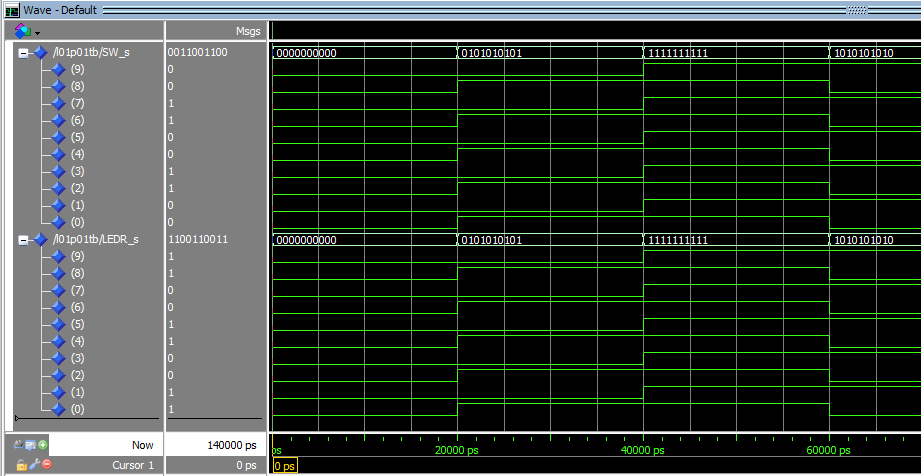
\includegraphics[width=1\textwidth]{Figures/Part1_Sim1.png}
        \caption{First four values}
        \label{fig:T01sim1}
    \end{subfigure}
    \begin{subfigure}{1\textwidth}
        \centering
        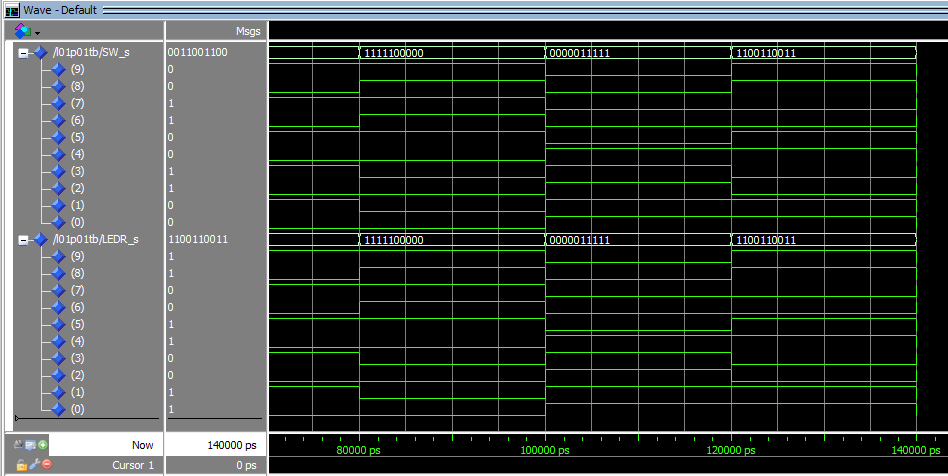
\includegraphics[width=1\textwidth]{Figures/Part1_Sim2.png}
        \caption{Next three values}
        \label{fig:T01sim2}
    \end{subfigure}
    \caption{Simulation results}
    \label{fig:T01sim}
\end{figure}
These are the simulation results. A keen eye might notice that the last value of the testbench is not diplayed. The issue is suspected to be that the wait command halts the simulation and the last chosen value will not be seen, for future simulations I will add an extra \verb|wait for 20 ns;| at the end to ensure the last value also gets tested. Due to the low importance of this last simulation result, redoing it has been omitted.


%   ############################## Section ##############################
\section{Task number 2}
This task was to write a simple 2-to-1 multiplexer. With two 4 bit inputs and a single selection bit and one 4 bit output. As the task supplied the statement that would add this functionality it relatively simple to program. Then I made a testbench code to test some inputs and see how it affected the outputs. In total 9 input combinations were tested. As LED nr 9 was used for a flag to see whether or not the selection input was on, the LEDs nr. 4-8 would not be in use and therefore they are assigned an unused signal such that they will not show up in the simulation.

\subsection{Code}
\writecode[VHDL]{Part2_Code.vhd}{TLE for a 4 bit 2 to 1 multiplexer}
\clearpage
\writecode[VHDL]{Part2_TB.vhd}{TestBench for the multiplexer}
\clearpage

\subsection{Simulation results}
\begin{figure}[h]
    \centering
    \begin{subfigure}{1\textwidth}
        \centering
        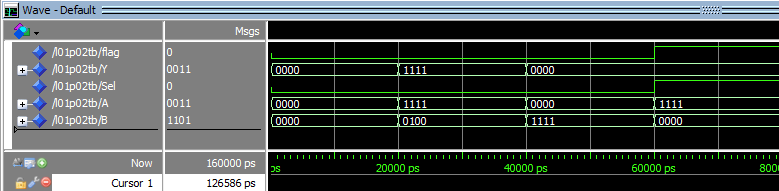
\includegraphics[width=1\textwidth]{Figures/Part2_Sim1.png}
        \caption{First four values}
        \label{fig:T02sim1}
    \end{subfigure}
    \begin{subfigure}{1\textwidth}
        \centering
        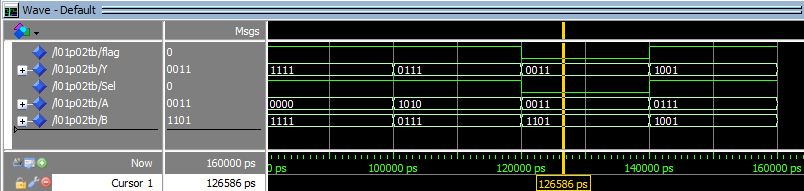
\includegraphics[width=1\textwidth]{Figures/Part2_Sim2.png}
        \caption{Next four values}
        \label{fig:T02sim2}
    \end{subfigure}
    \caption{Simulation results}
    \label{fig:T02sim}
\end{figure}
Here you can see that the output is as expected. As long as Sel is set to 0 the flag is set to 0 and the output, Y is equal to input A. Then Sel is switched to 1 and that makes flag also go to 1 and output Y is now equal to input B instead. With the same reasoning as previous task the last line of test values are not shown, and screenshots will not be redone for this task either.


%   ############################## Section ##############################
\section{Task number 3}
This task was similar to the previous but this time a 4-to-1 multiplexer. With four 2 bit inputs and a 2 bit selection and one 2 bit output. The logic statements from the previous task were used on two separate 2-to-1 multiplexers and results stored in a signal, where the final output was a 2-to-1 multiplexing of the signals. This then made up the 4-to-1 multiplexer.  Then I made a testbench code to test some inputs and see how it affected the outputs. In total 8 input combinations were tested.

\subsection{Code}
\writecode[VHDL]{Part3_Code.vhd}{TLE for a 2 bit 4 to 1 multiplexer}
\clearpage
\writecode[VHDL]{Part3_TB.vhd}{TestBench for the multiplexer}
\clearpage

\subsection{Simulation results}
\begin{figure}[h]
    \centering
    \begin{subfigure}{1\textwidth}
        \centering
        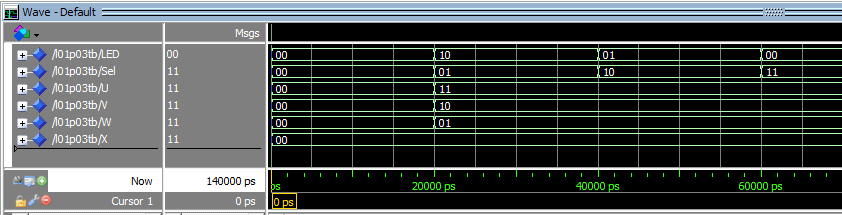
\includegraphics[width=1\textwidth]{Figures/Part3_Sim1.png}
        \caption{First four values}
        \label{fig:T03sim1}
    \end{subfigure}
    \begin{subfigure}{1\textwidth}
        \centering
        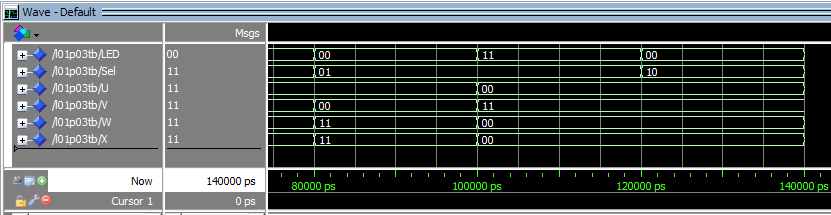
\includegraphics[width=1\textwidth]{Figures/Part3_Sim2.png}
        \caption{Next three values}
        \label{fig:T03sim2}
    \end{subfigure}
    \caption{Simulation results}
    \label{fig:T03sim}
\end{figure}
Here you can see that the output is as expected. When Sel is set to 00 the output, LED is equal to input U. When Sel is set to 01 the output is equal to input V. When Sel is set to 10 the output is equal to input W. When Sel is set to 11 the output is equal to input X. With the same reasoning as both previous tasks, the last line of test values are not shown, and screenshots will not be redone for this task either.


%   ############################## Section ##############################
\section{Task number 4}
This task was to make a simple decoder for a 7 segment display. It would have a 2 bit input and a 7 bit output with the possibility to display "d", "E", "1" or off depending on the input. First I started with finding the boolean expression needed and then simply made a structural architecture based on the expressions for each output. Then it was tested on a FPGA board to show that it worked as expected.

\subsection{Boolean expression}
To find the boolean expressions I could have calculated it manual using boolean algebra but instead I oped for a truth table to expression solver to save time as there was no point in doing it manual. For segments 1-4 and 6 I saw there was a simple relation, just depending on one of the inputs and those were just used diractly, for the few segments with a bit more advanced relation I used \url{https://tma.main.jp/logic/index_en.html} to find the simplified boolean expression from the truth table.

\subsection{Code}
\writecode[VHDL]{Part4_Code.vhd}{TLE for a simple 7 segment decoder}
\clearpage

\subsection{RTL}
\begin{figure}[h]
    \centering
    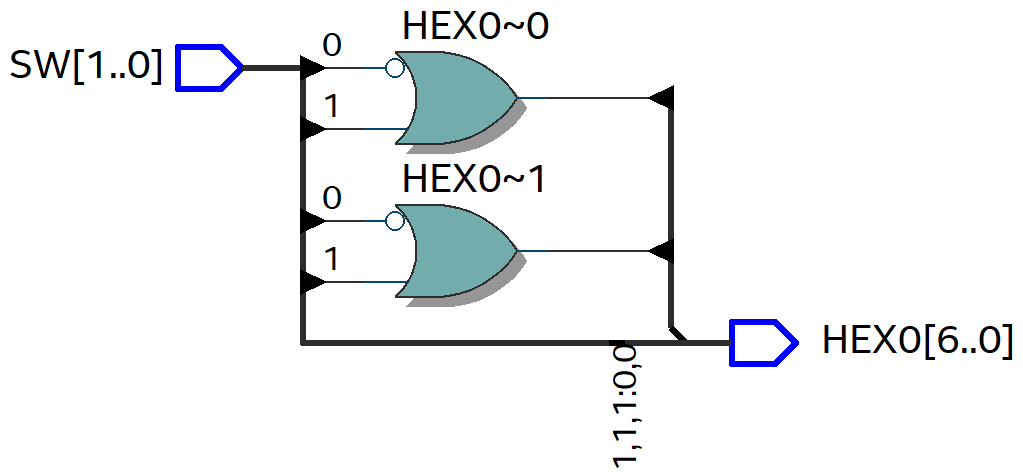
\includegraphics[width=1\textwidth]{Figures/Part4_RTL.png}
    \caption{RTL synthesizing of the circuit}
    \label{fig:T04rtl}
\end{figure}
It is not clear from the RTL view what input is connected to witch segments. Based on the numbering near the bottom, you can see that two instances of SW[0] is connected directly and three instances of SW[1]. Two segments are connected to each an or gate that is connected to SW[1] on one input and inverted SW[0]. This fits logically with what the code is doing, although there was no need to use two gates as the outputs are equal and could be connected together directly. 
\clearpage

\subsection{Results}
\begin{figure}[h]
    \centering
    \begin{subfigure}{0.4\textwidth}
        \centering
        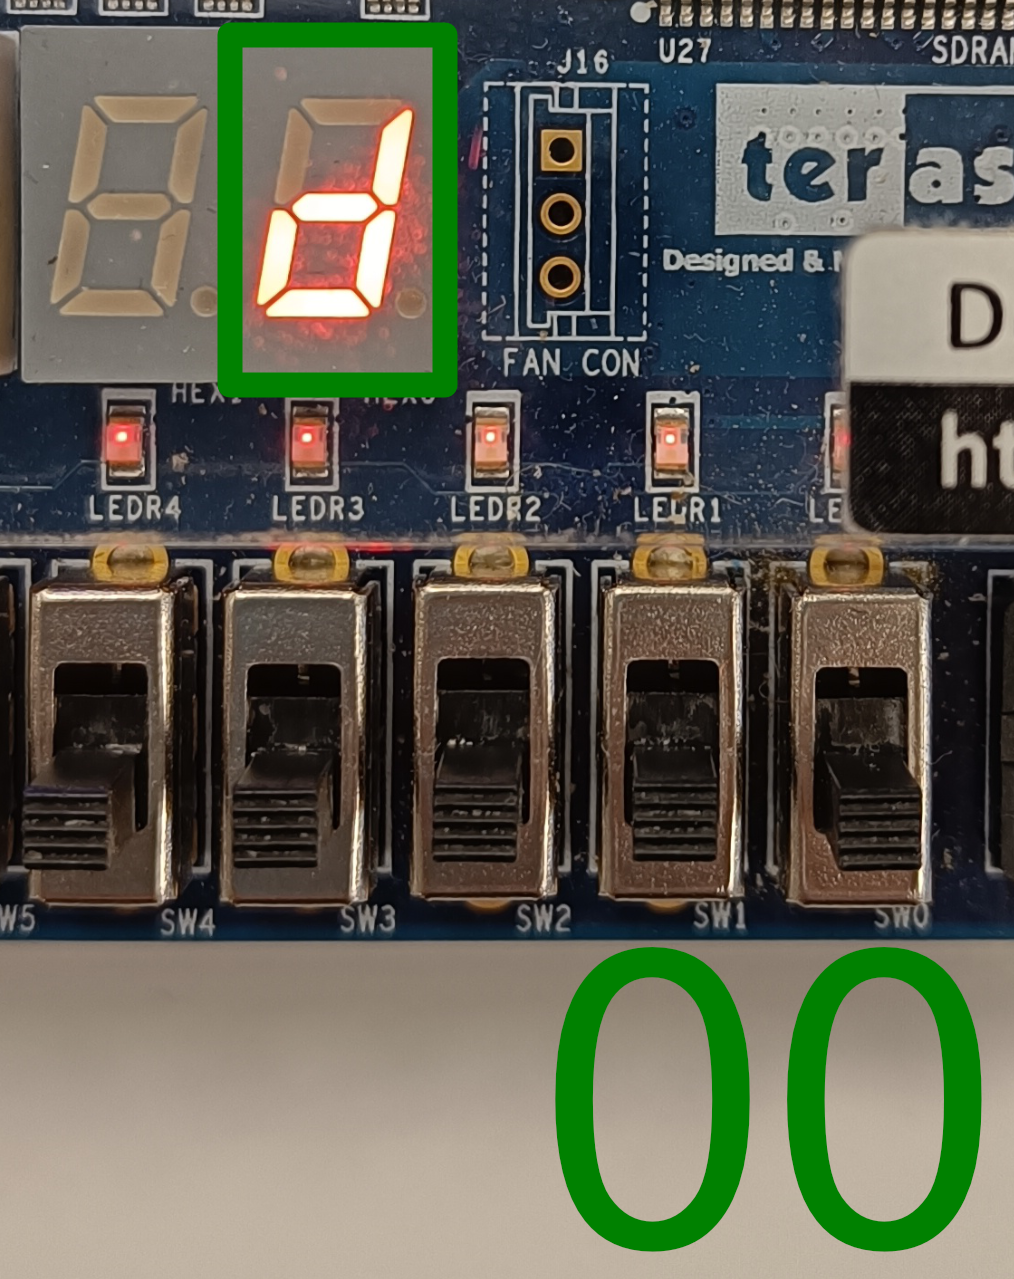
\includegraphics[width=1\textwidth]{Figures/Part4-00.png}
        \caption{"d" at 00}
        \label{fig:T04pic1}
    \end{subfigure}
    \hfill
    \begin{subfigure}{0.4\textwidth}
        \centering
        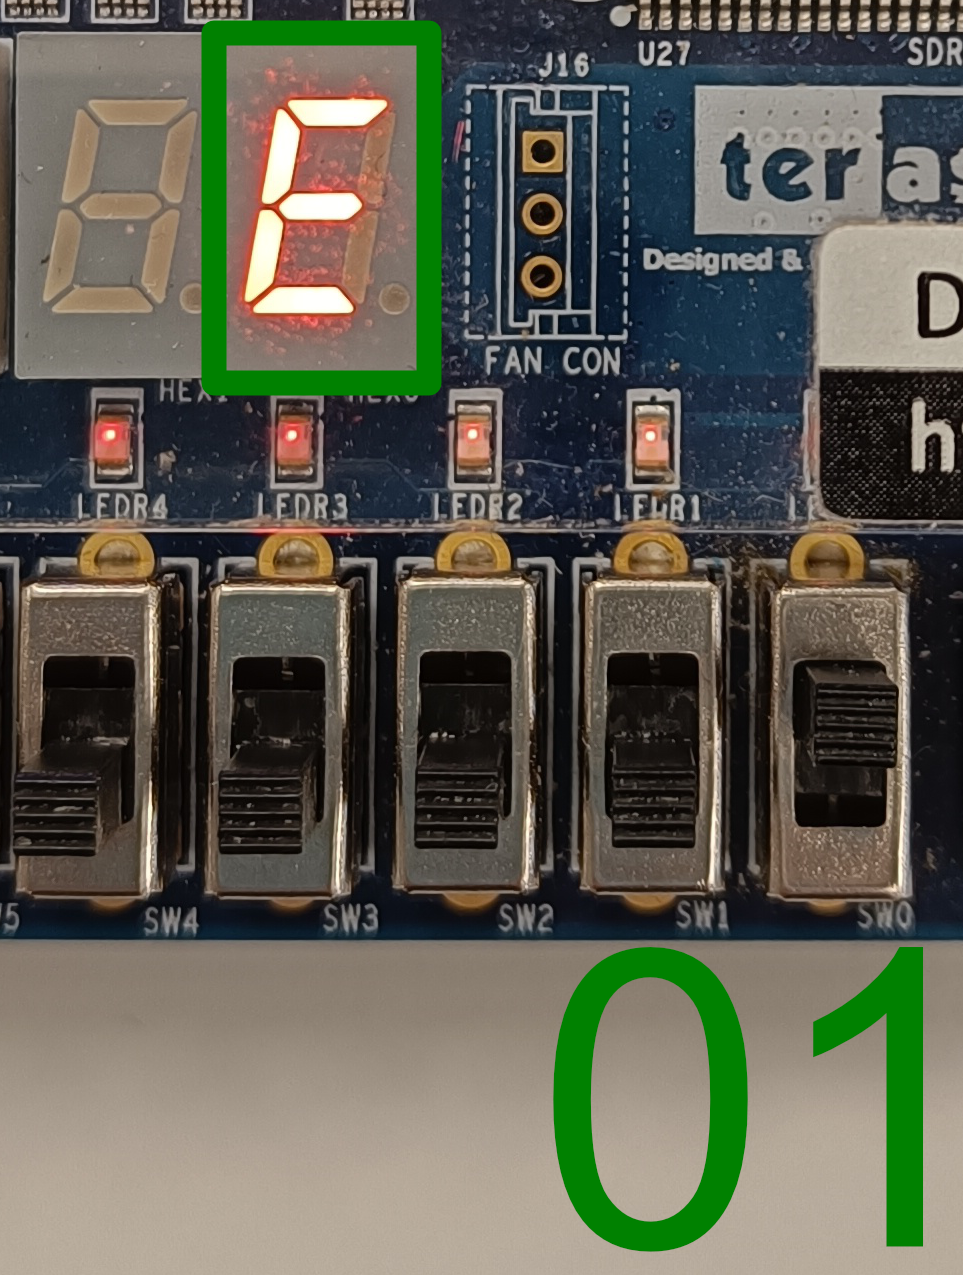
\includegraphics[width=1\textwidth]{Figures/Part4-01.png}
        \caption{"E" at 01}
        \label{fig:T04pic2}
    \end{subfigure}
    \begin{subfigure}{0.4\textwidth}
        \centering
        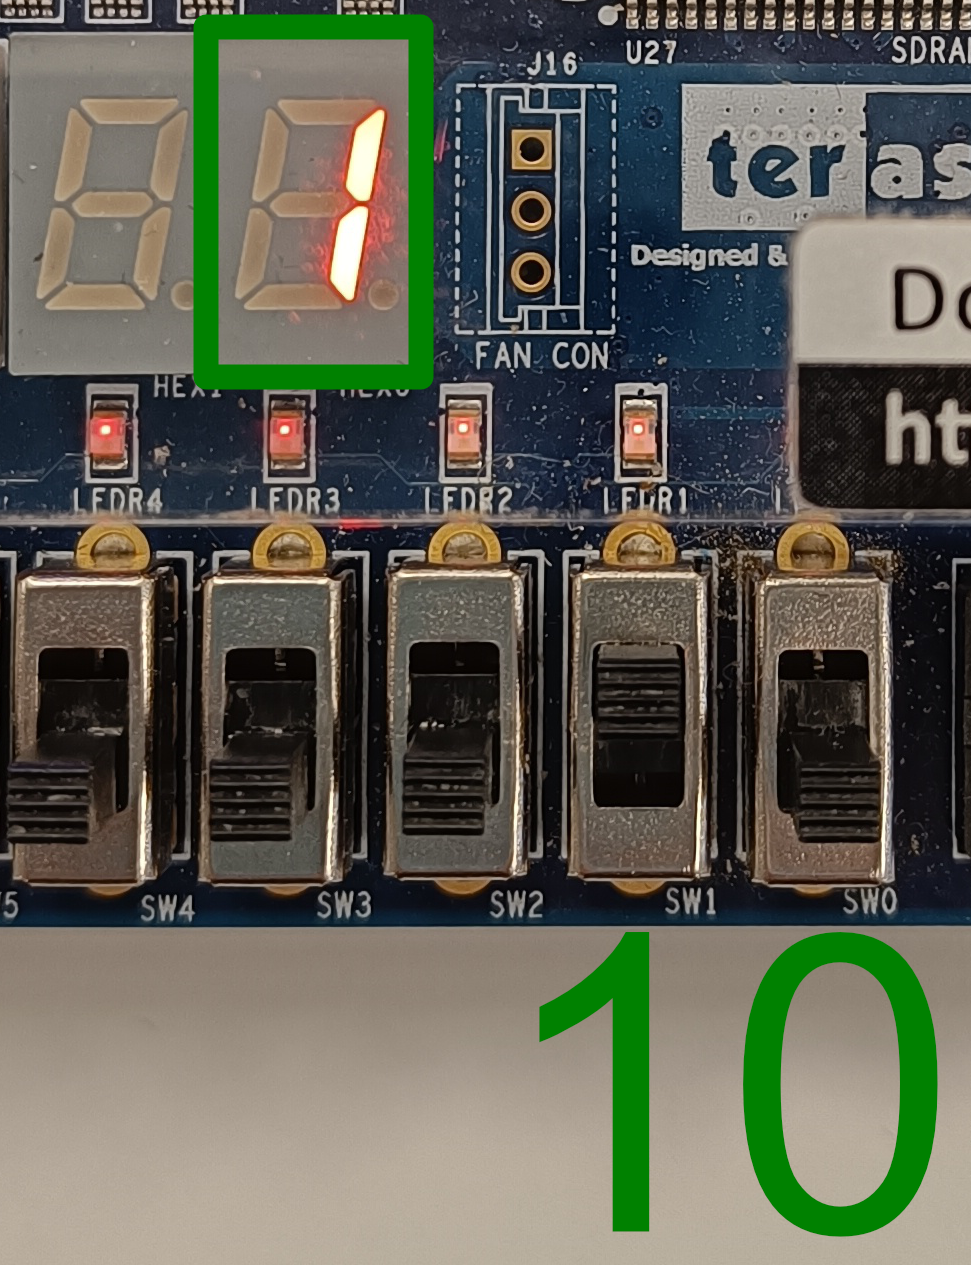
\includegraphics[width=1\textwidth]{Figures/Part4-10.png}
        \caption{"1" at 10}
        \label{fig:T04pic3}
    \end{subfigure}
    \hfill
    \begin{subfigure}{0.4\textwidth}
        \centering
        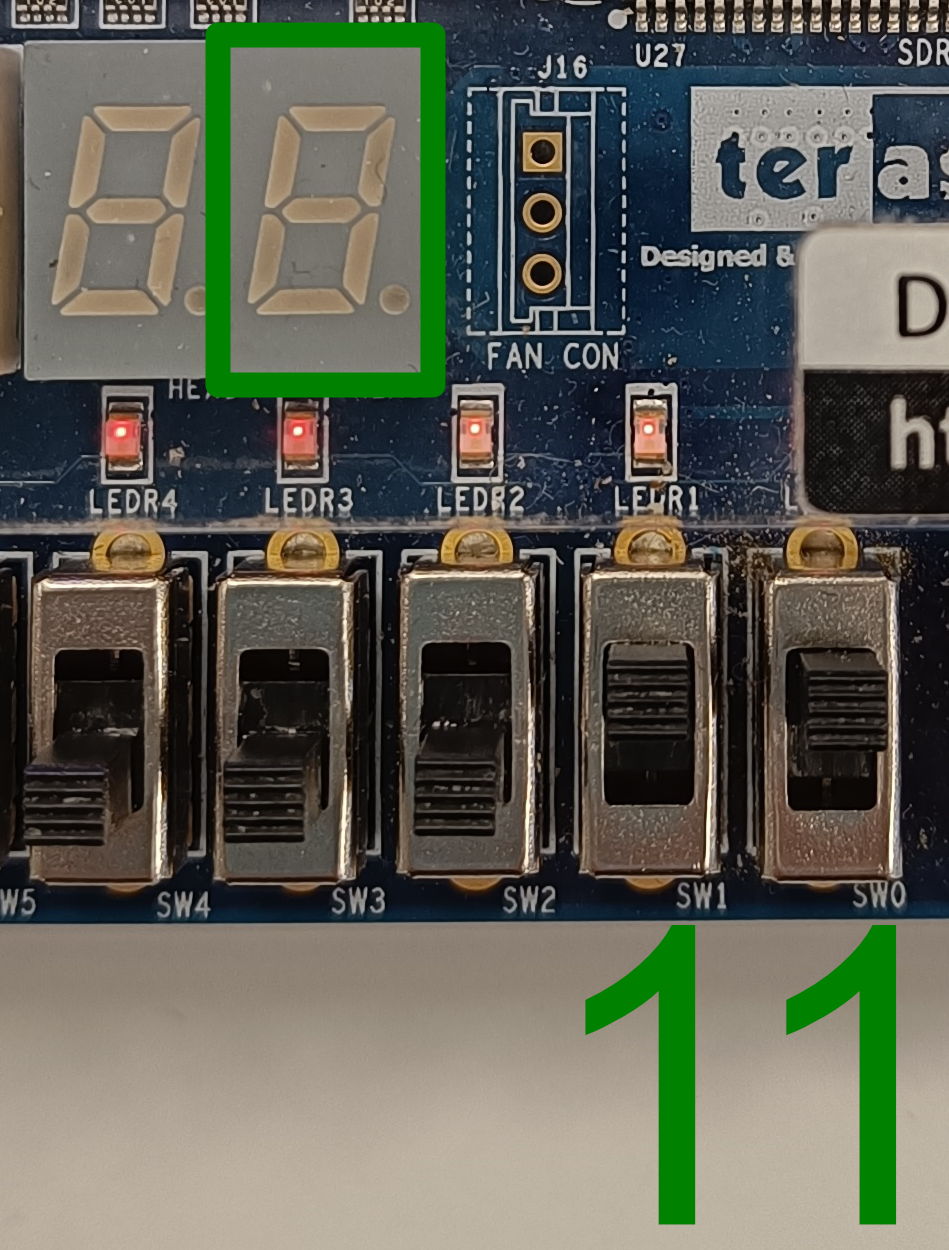
\includegraphics[width=1\textwidth]{Figures/Part4_11.png}
        \caption{off at 11}
        \label{fig:T04pic4}
    \end{subfigure}
    \caption{Test results}
    \label{fig:T04pic}
\end{figure}
Here you can see that the output is as expected. When the input is set to 00 the output is the letter "d". When the input is set to 01 the output is the letter "E". When the input is set to 10 the output is the number "1". When the input is set to 11 the output is off.

%   ############################## Section ##############################
\section{Task number 5}
This is the final task for this lab and it was to combine the 2 bit 4-to-1 multiplexer with the 2 bit 7 segment display encoder. And rotated for 4 displays, such that the first display gets the first input, the second display gets the second input, third gets third and fourth gets fourth. Then when changing the selection input everything would rotate to the display next to it, and the last would wrap around to the first. I started with making the code for a 2 bit 4-to-1 multiplexer, very similar as in part 3. Then I made the code to a 2 bit decoder to a 7 segment display, very similar to part 4. Finally I made a TLE(Top Level Entity) code that imported the two previous codes. The TLE is constructed with four instances of the multiplexer to have one for each display, with the inputs rotated, such that if selection is 00 the output would be the first input on the left most display, the second input on the next display and so on. Four instances of the encoder was also added such that all 4 displays got their own encoder. As an extra feature, described in the task, all the switch inputs should light up each corresponding led to easier show on off position easier in pictures. After this the code was uploaded to a FPGA board and tested.

\subsection{Code}
\writecode[VHDL]{Part5_Code_mux.vhd}{2 bit 4-to-1 multiplexer}
\clearpage
\writecode[VHDL]{Part5_Code_decoder.vhd}{2 bit 7 segment decoder}
\clearpage
\writecode[VHDL]{Part5_Code_TLE.vhd}{TLE for rotating display}
\clearpage

\subsection{RTL}
\begin{figure}[h]
    \centering
    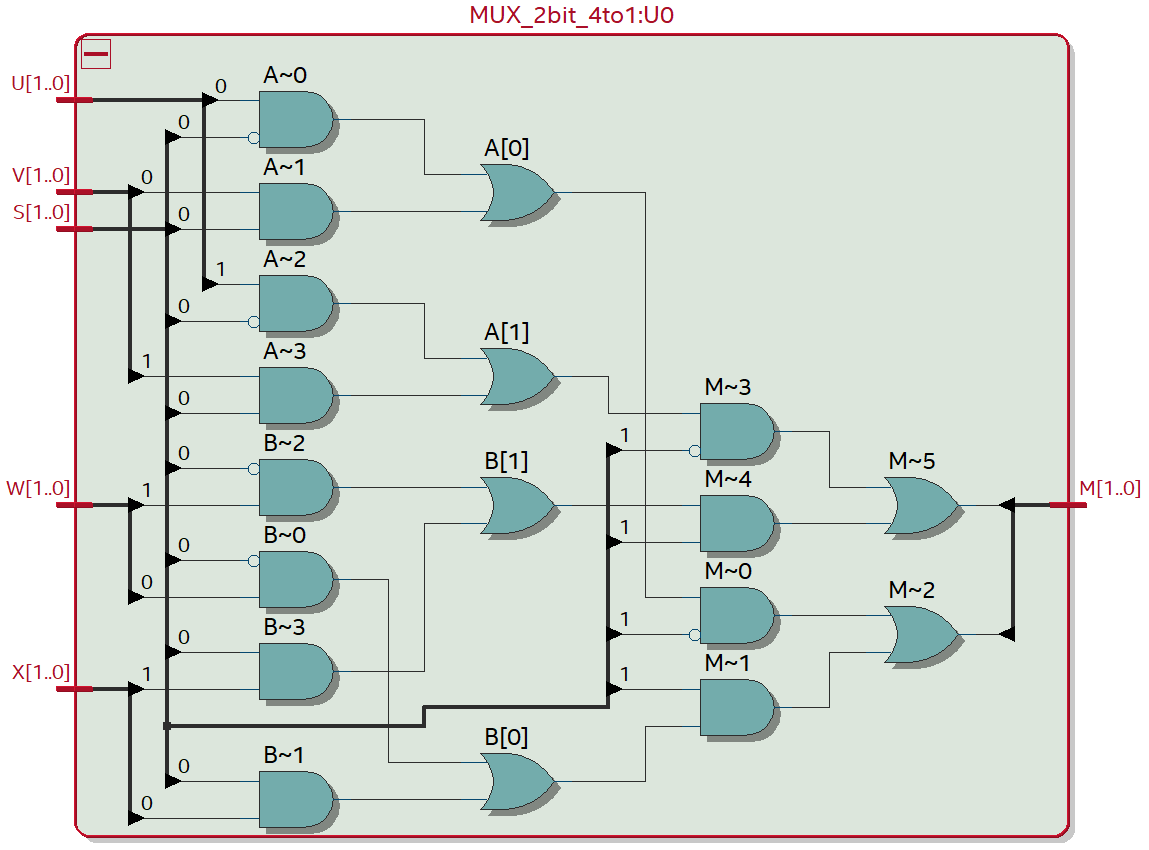
\includegraphics[width=1\textwidth]{Figures/Part5_RTL_mux.png}
    \caption{RTL synthesizing of the multiplexer circuit}
    \label{fig:T05rtlmux}
\end{figure}
This is the RTL view of the first of the four instances of the multiplexer. If part 3 were synthesized it would look pretty close as it is the same logic used in both circus. Here you can see that the inputs are the U, V, W, X and the selector input S, all of which are 2 bit. and the output is the 2 bit M.\par
\begin{figure}[h]
    \centering
    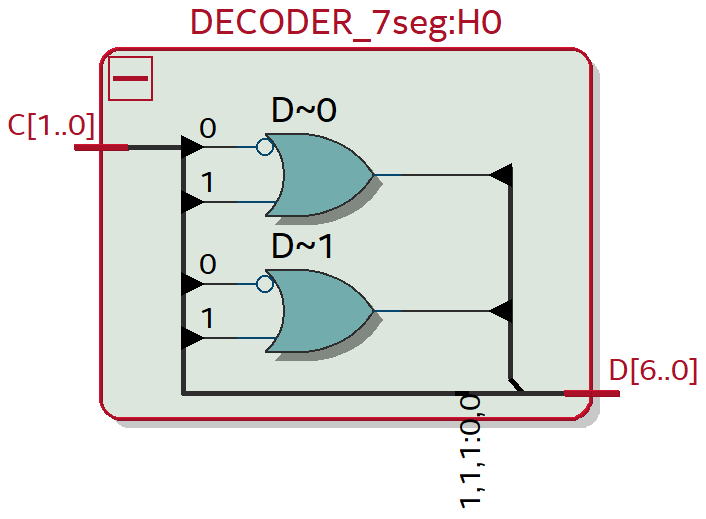
\includegraphics[width=0.4\textwidth]{Figures/Part5_RTL_decoder.png}
    \caption{RTL synthesizing of the decoder circuit}
    \label{fig:T05rtldecoder}
\end{figure}
This is the exact same function as the RTL in task 4 shows, as the codes are nearly identical.
\clearpage
\begin{figure}[h]
    \centering
    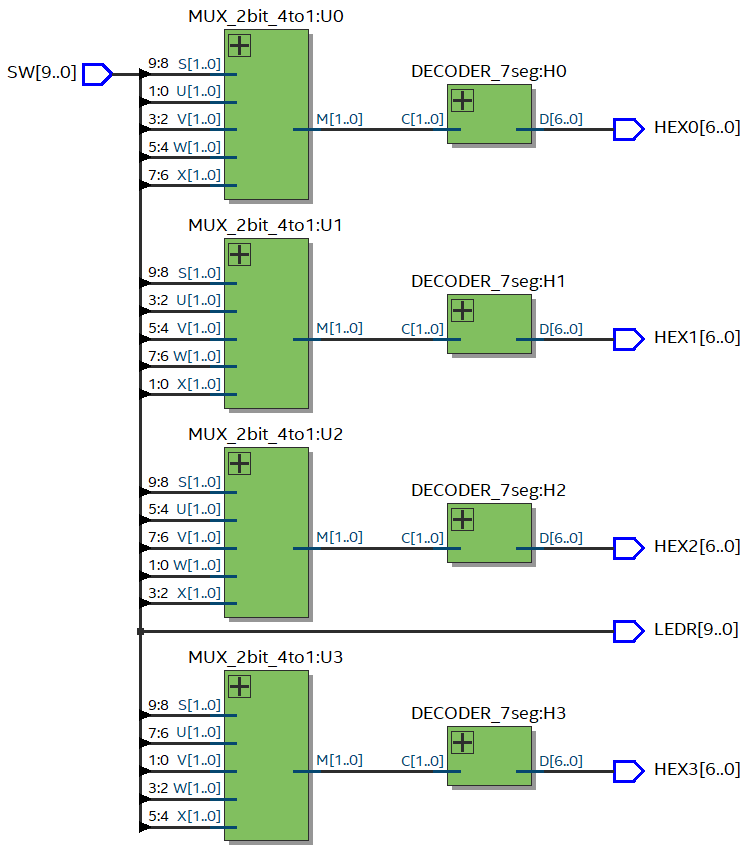
\includegraphics[width=1\textwidth]{Figures/Part5_TRL_TLE.png}
    \caption{RTL synthesizing of the TLE circuit}
    \label{fig:T05rtltle}
\end{figure}
Here the setup of how each multiplexer is connected to each decoder that is connected to its own display is quite clear. You can also see on the input numbering that the numbers leading into each U, V, W and X on each multiplexer is rotating through the instances. Here you also see that the switches directly control the LEDs as well.
\clearpage

\subsection{Results}
\begin{figure}[h]
    \centering
    \begin{subfigure}{0.45\textwidth}
        \centering
        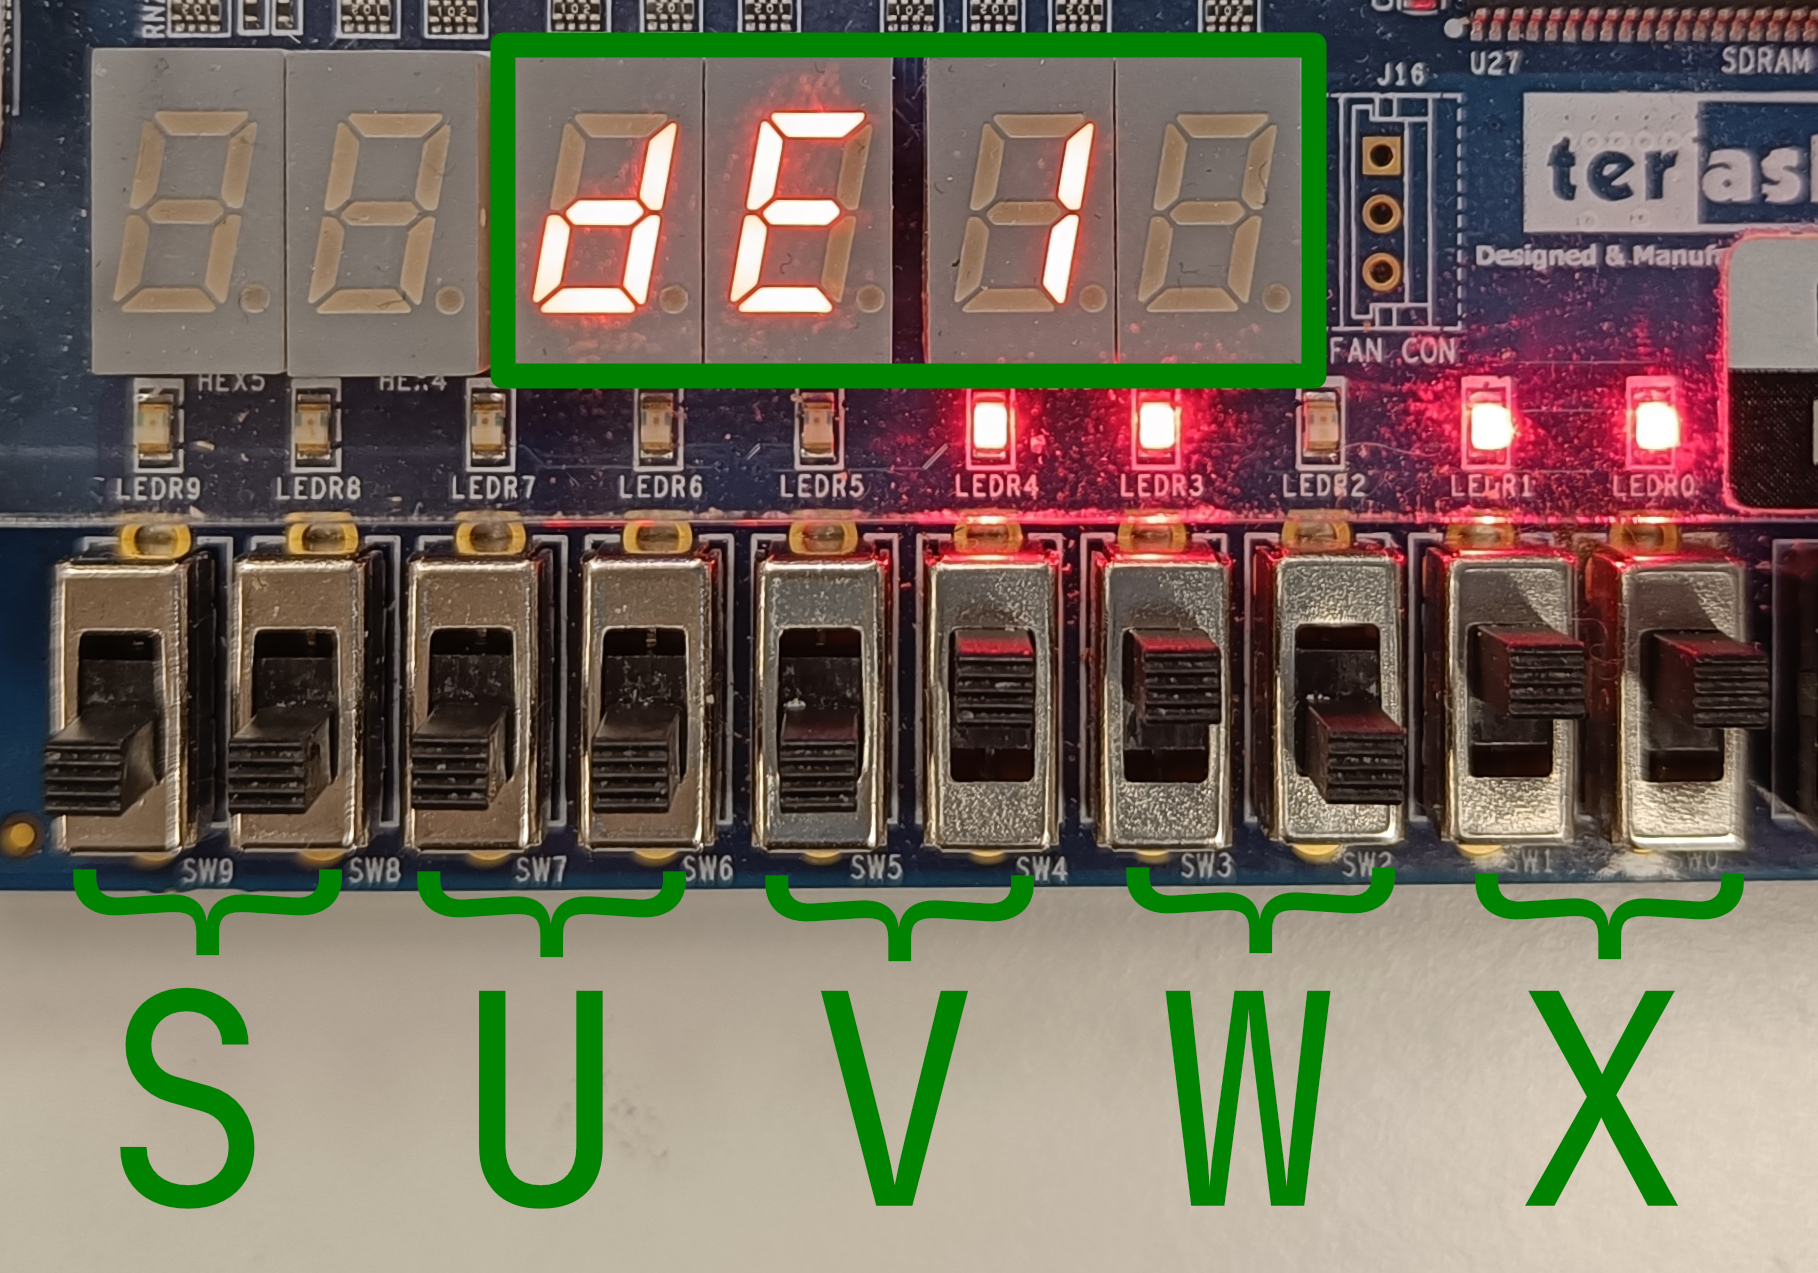
\includegraphics[width=1\textwidth]{Figures/Part5_dE1_00.png}
        \caption{"dE1 " at S = 00}
        \label{fig:T05de1pic1}
    \end{subfigure}
    \hfill
    \begin{subfigure}{0.45\textwidth}
        \centering
        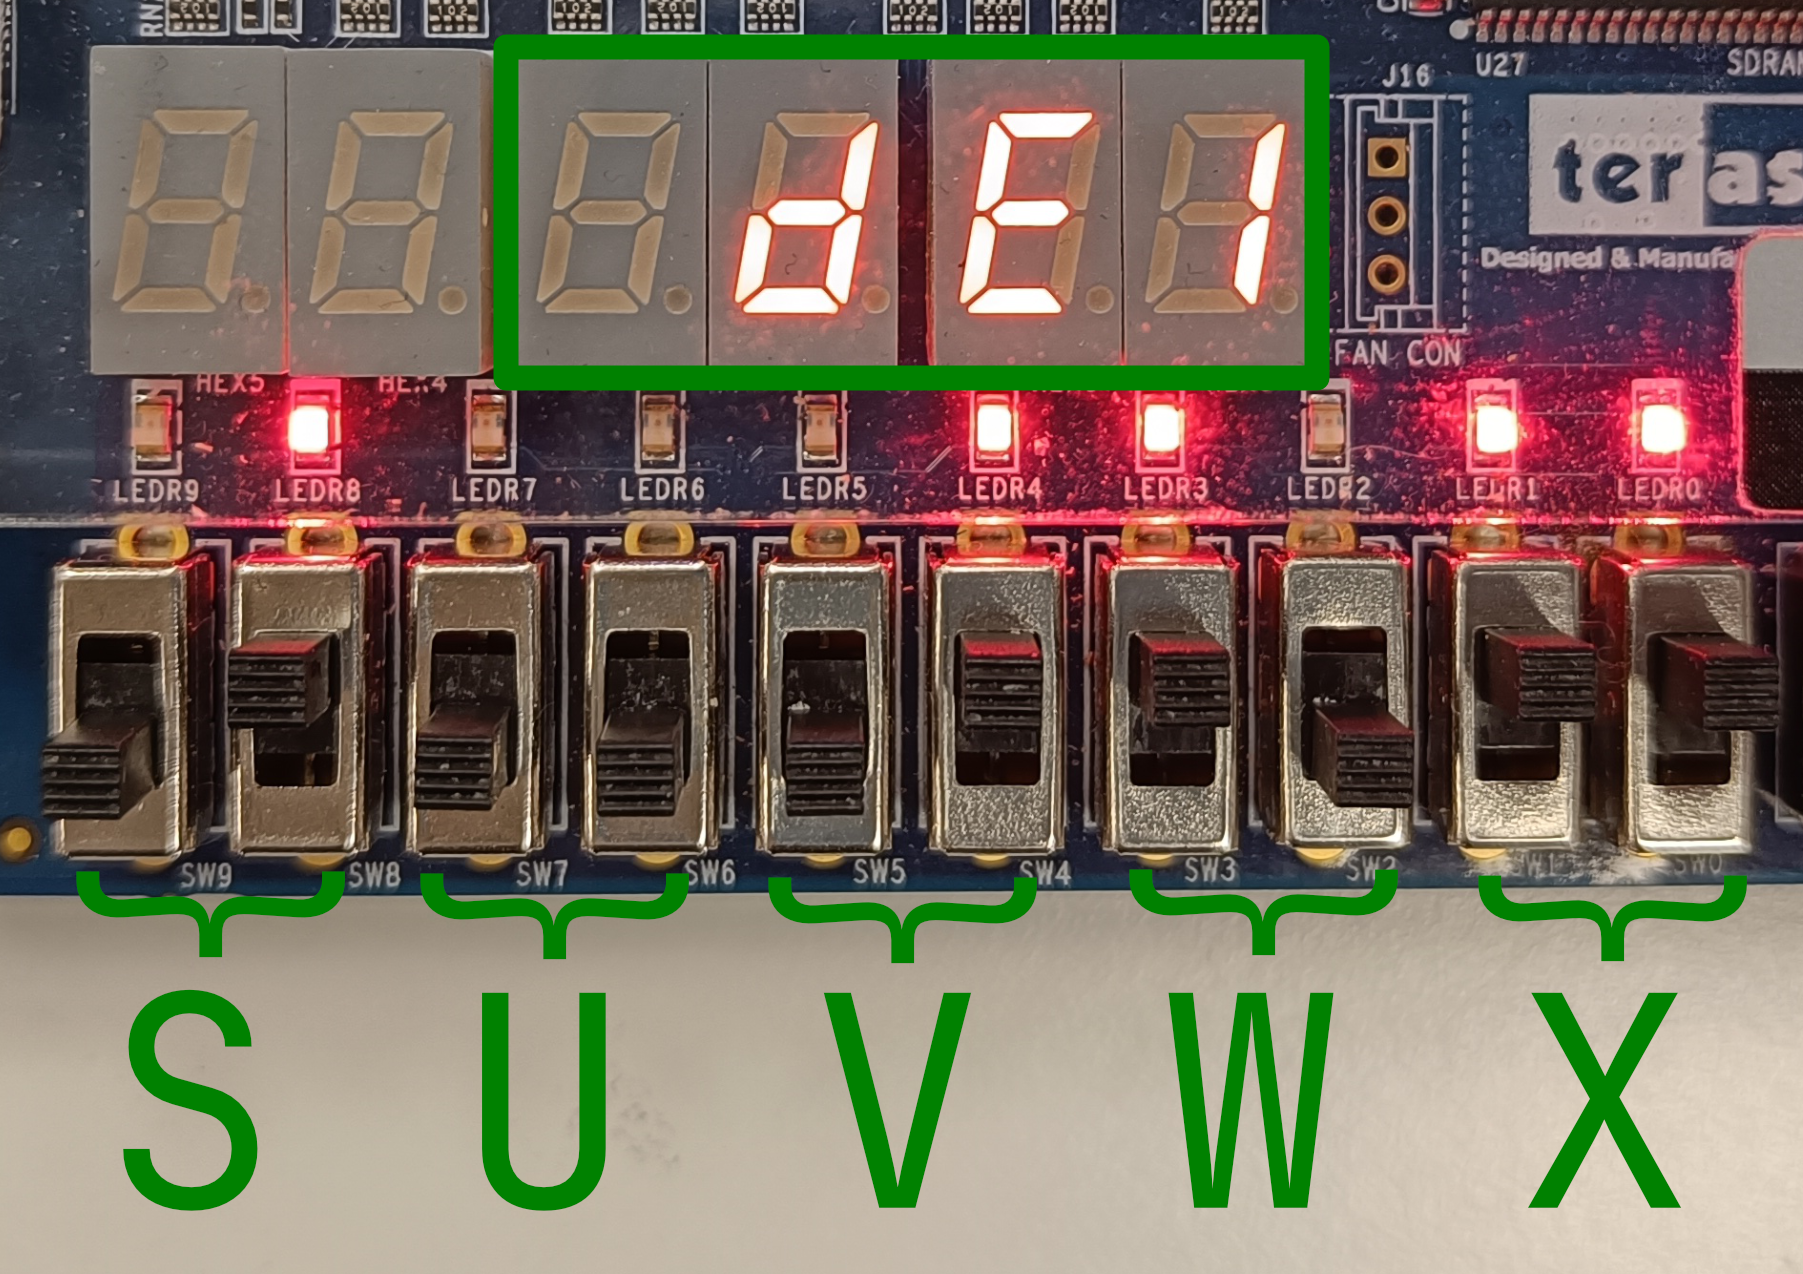
\includegraphics[width=1\textwidth]{Figures/Part5_dE1_01.png}
        \caption{" dE1" at S = 01}
        \label{fig:T05de1pic2}
    \end{subfigure}
    \begin{subfigure}{0.45\textwidth}
        \centering
        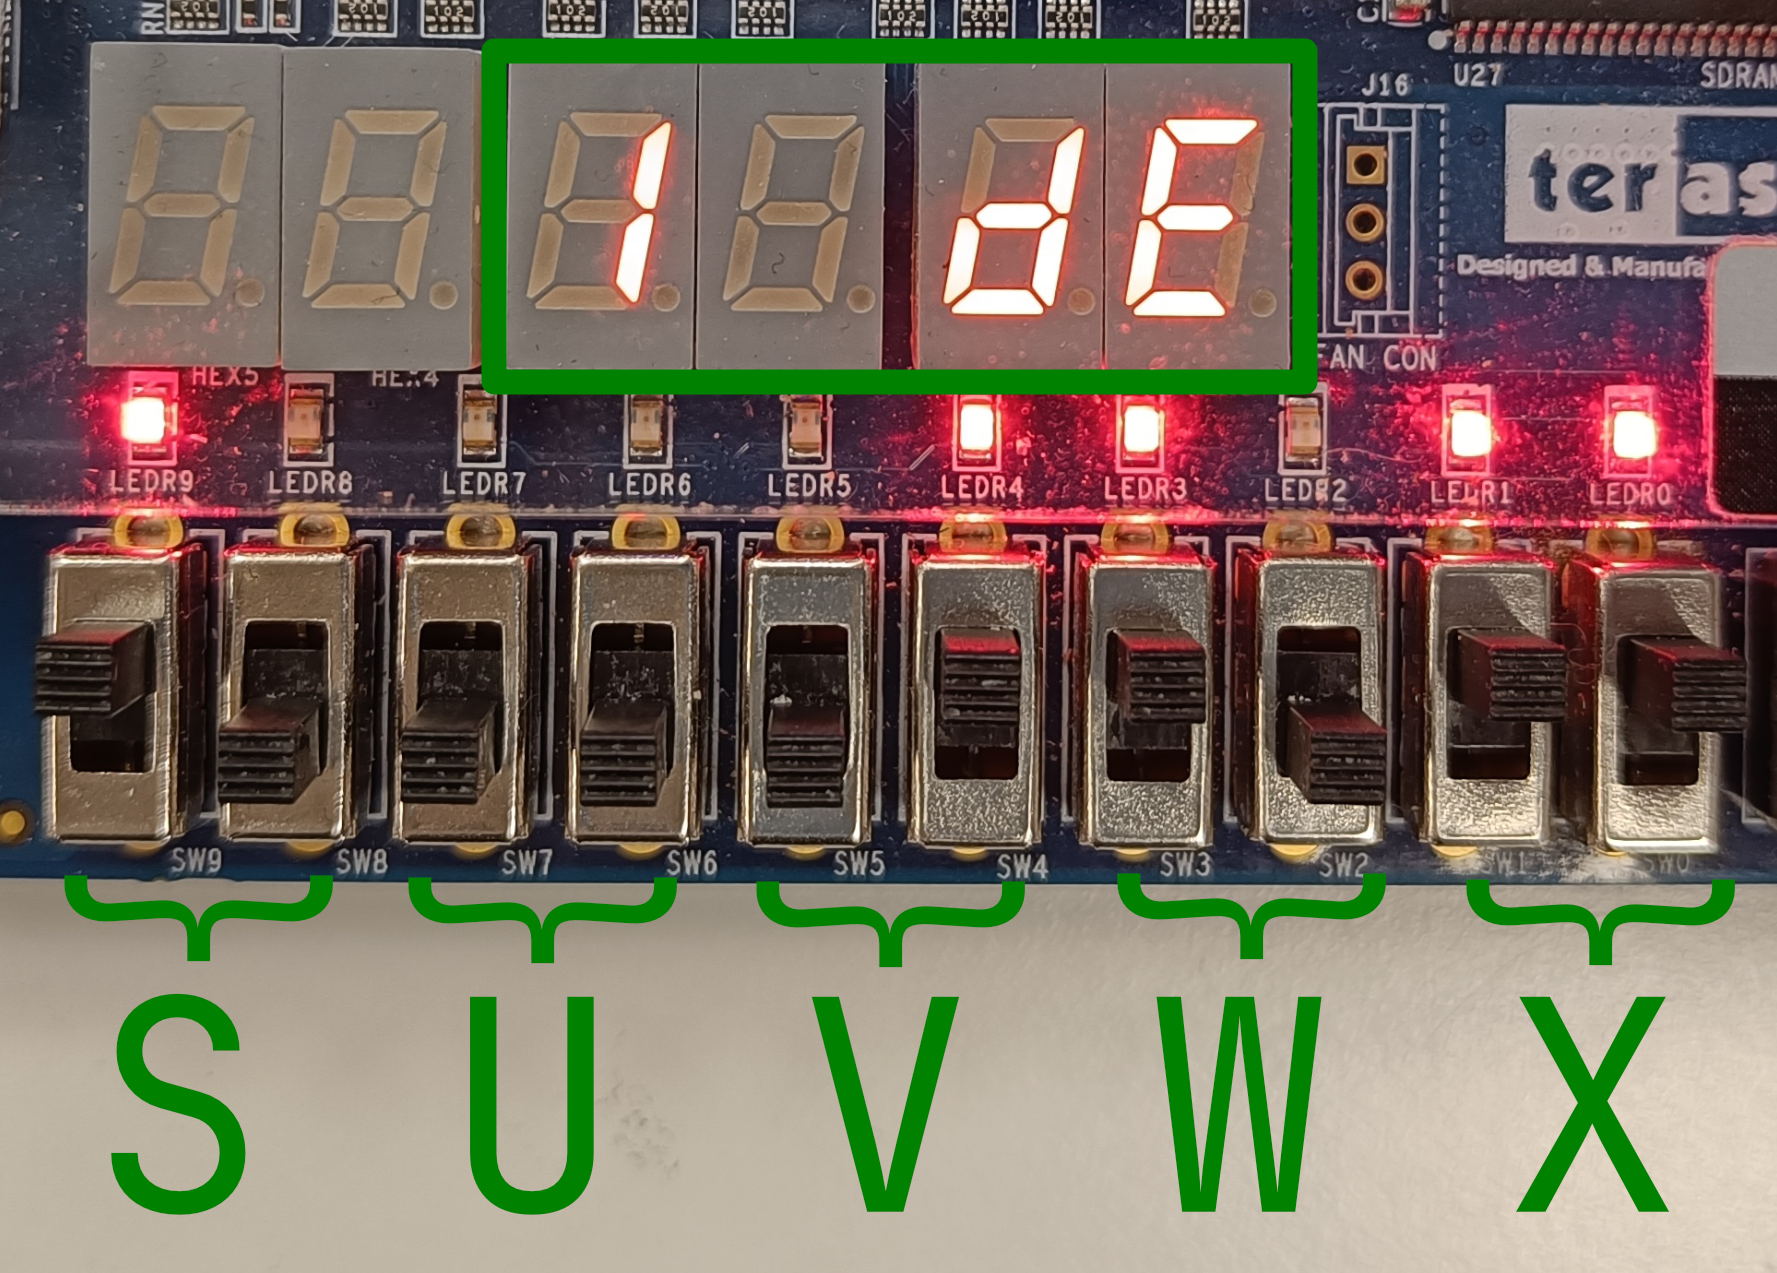
\includegraphics[width=1\textwidth]{Figures/Part5_dE1_10.png}
        \caption{"1 dE" at s = 10}
        \label{fig:T05de1pic3}
    \end{subfigure}
    \hfill
    \begin{subfigure}{0.45\textwidth}
        \centering
        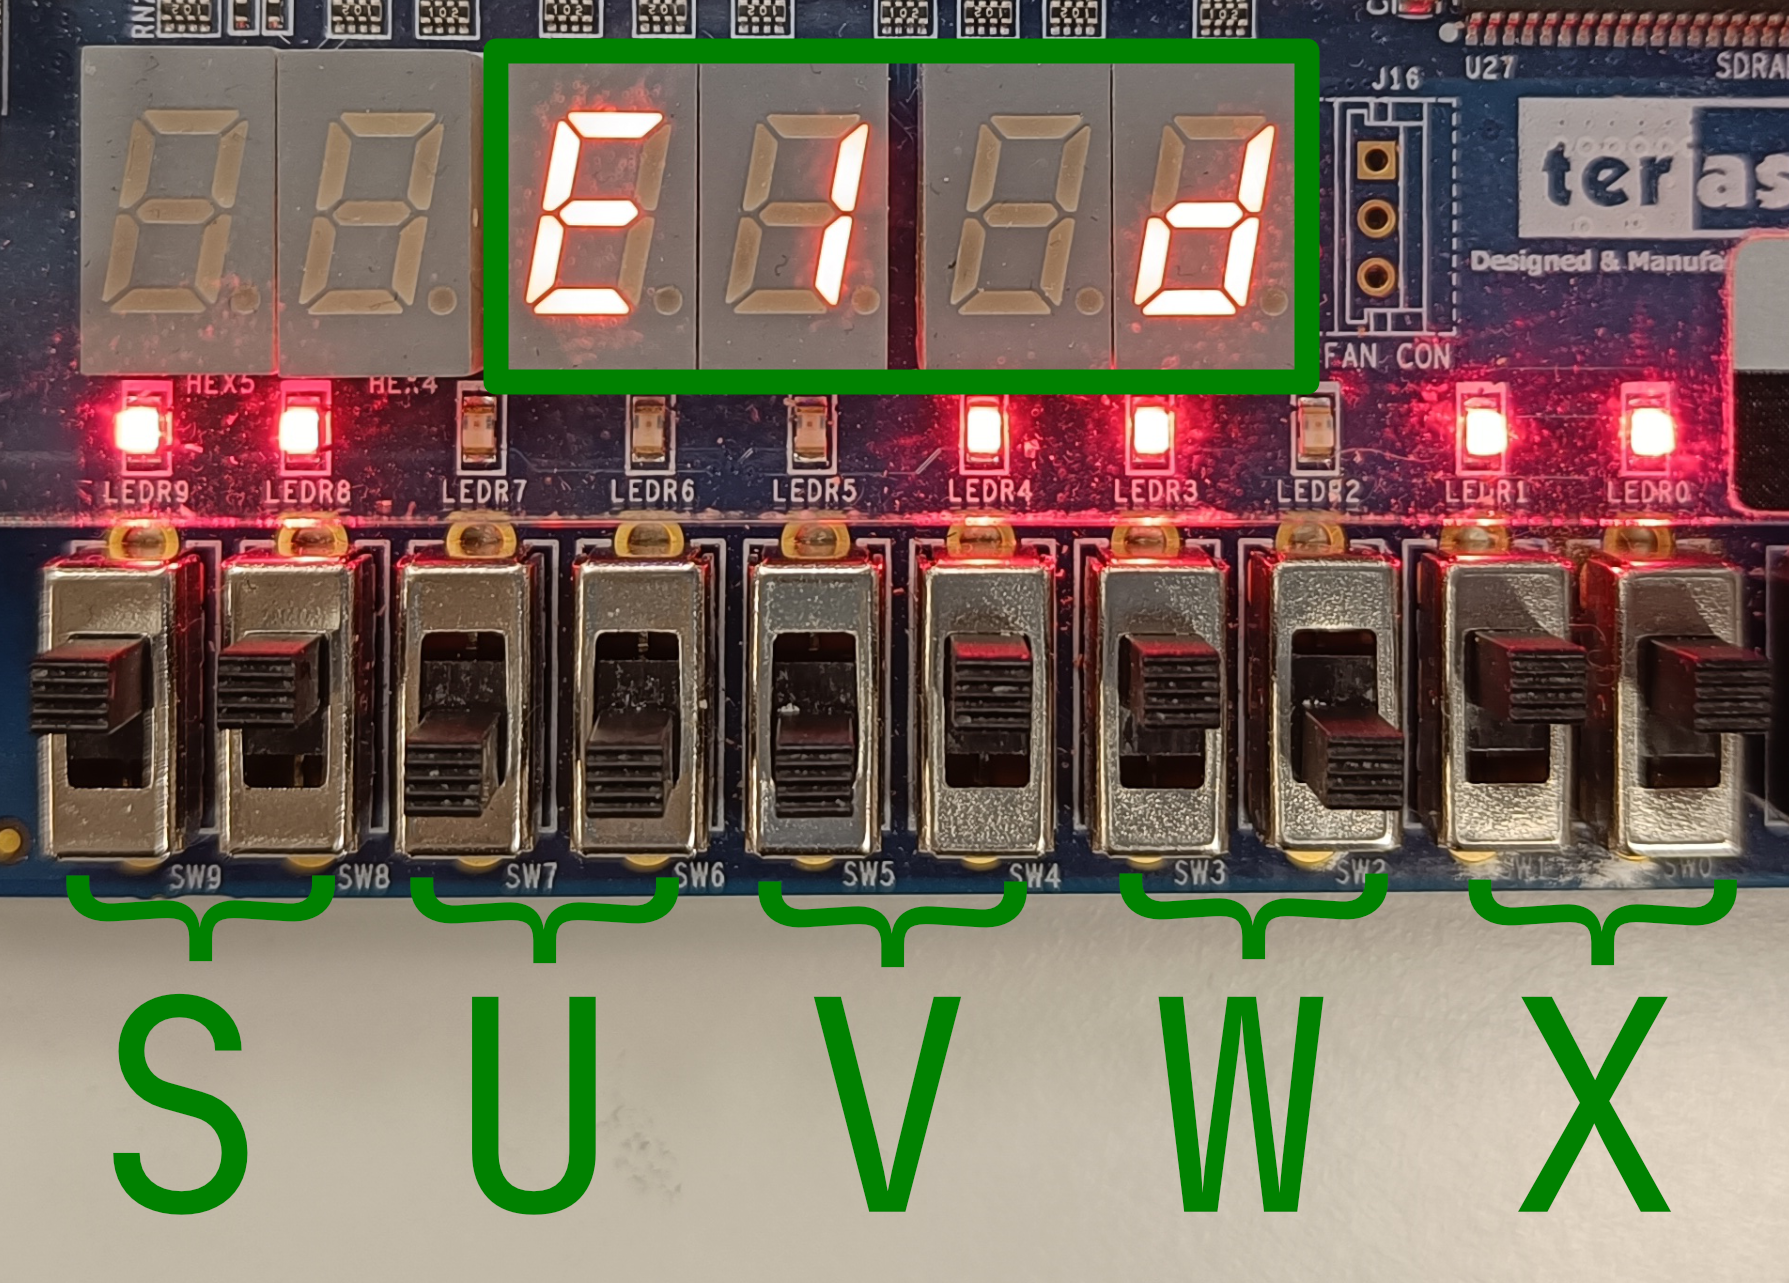
\includegraphics[width=1\textwidth]{Figures/Part5_dE1_11.png}
        \caption{"E1 d" at s = 11}
        \label{fig:T05de1pic4}
    \end{subfigure}
    \caption{Test results for "dE1 " input}
    \label{fig:T05de1pic}
\end{figure}
Here you can see that the only input changing is the selection and changing it makes the whole display rotate. The input for U is 00, which is for d, the input for V is  01 which is for E, the input for W is 10 which is for 1, and the input for X is 11 which is for off.
\clearpage
\begin{figure}[h]
    \centering
    \begin{subfigure}{0.45\textwidth}
        \centering
        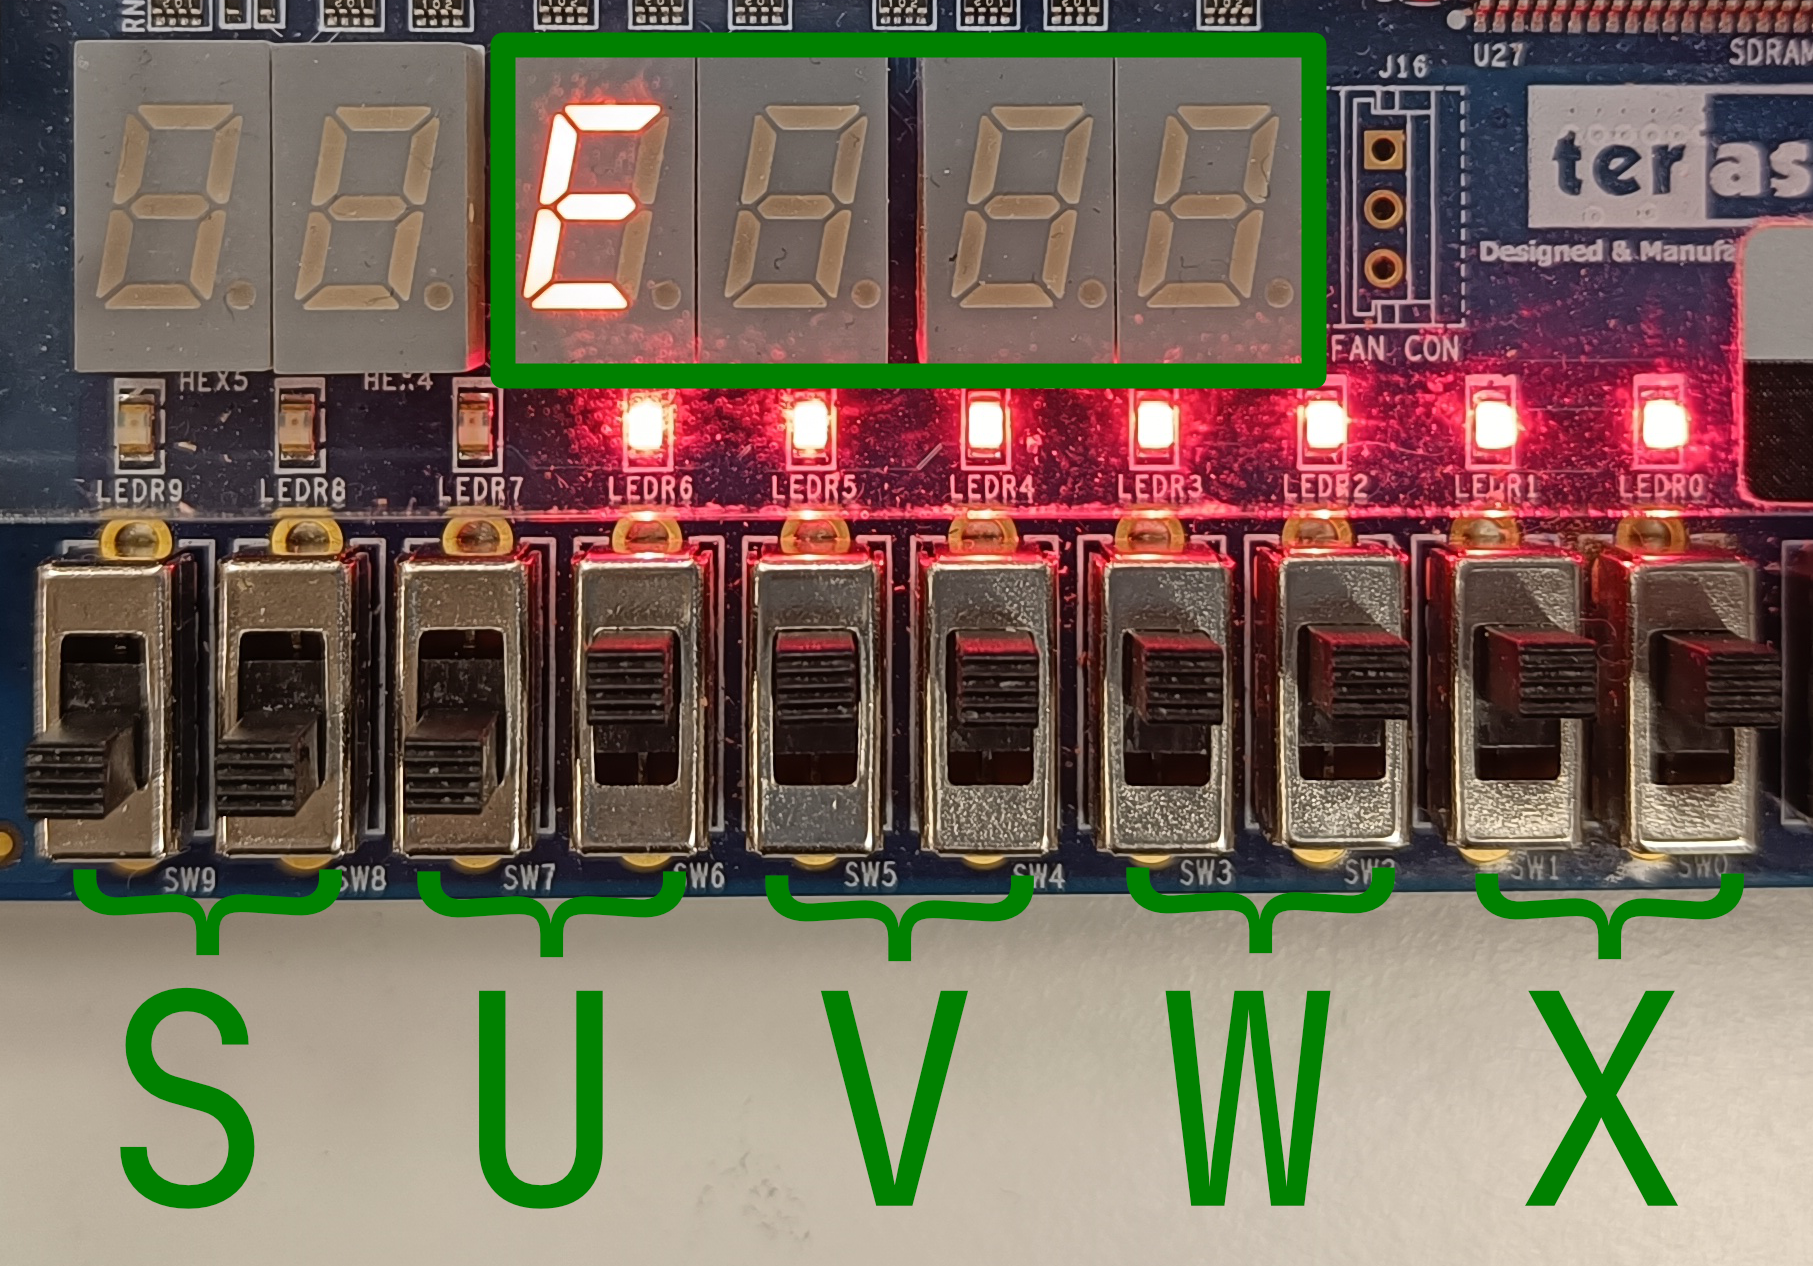
\includegraphics[width=1\textwidth]{Figures/Part5_E_00.png}
        \caption{E first at S = 00}
        \label{fig:T05epic1}
    \end{subfigure}
    \hfill
    \begin{subfigure}{0.45\textwidth}
        \centering
        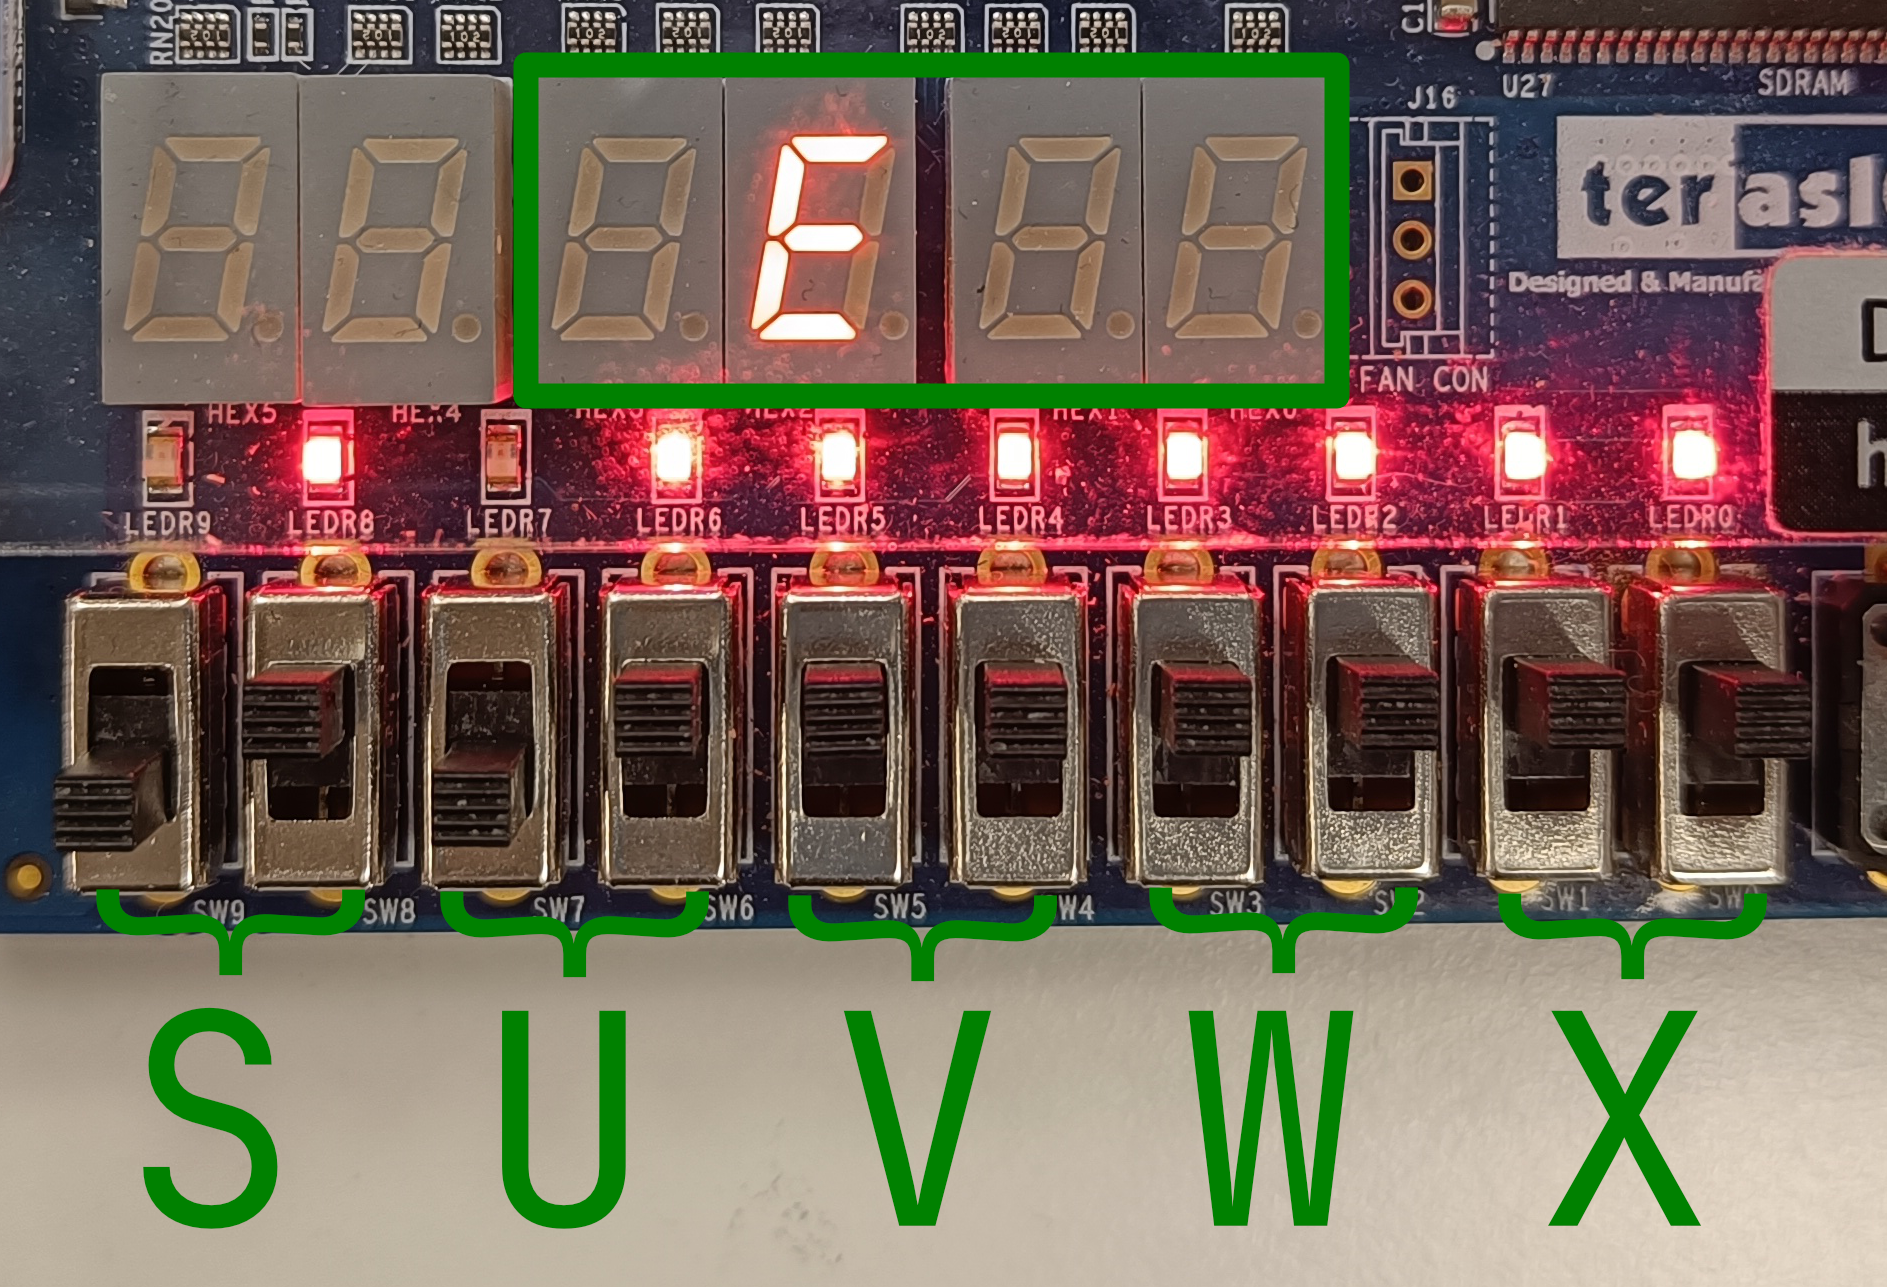
\includegraphics[width=1\textwidth]{Figures/Part5_E_01.png}
        \caption{E second at S = 01}
        \label{fig:T05epic2}
    \end{subfigure}
    \begin{subfigure}{0.45\textwidth}
        \centering
        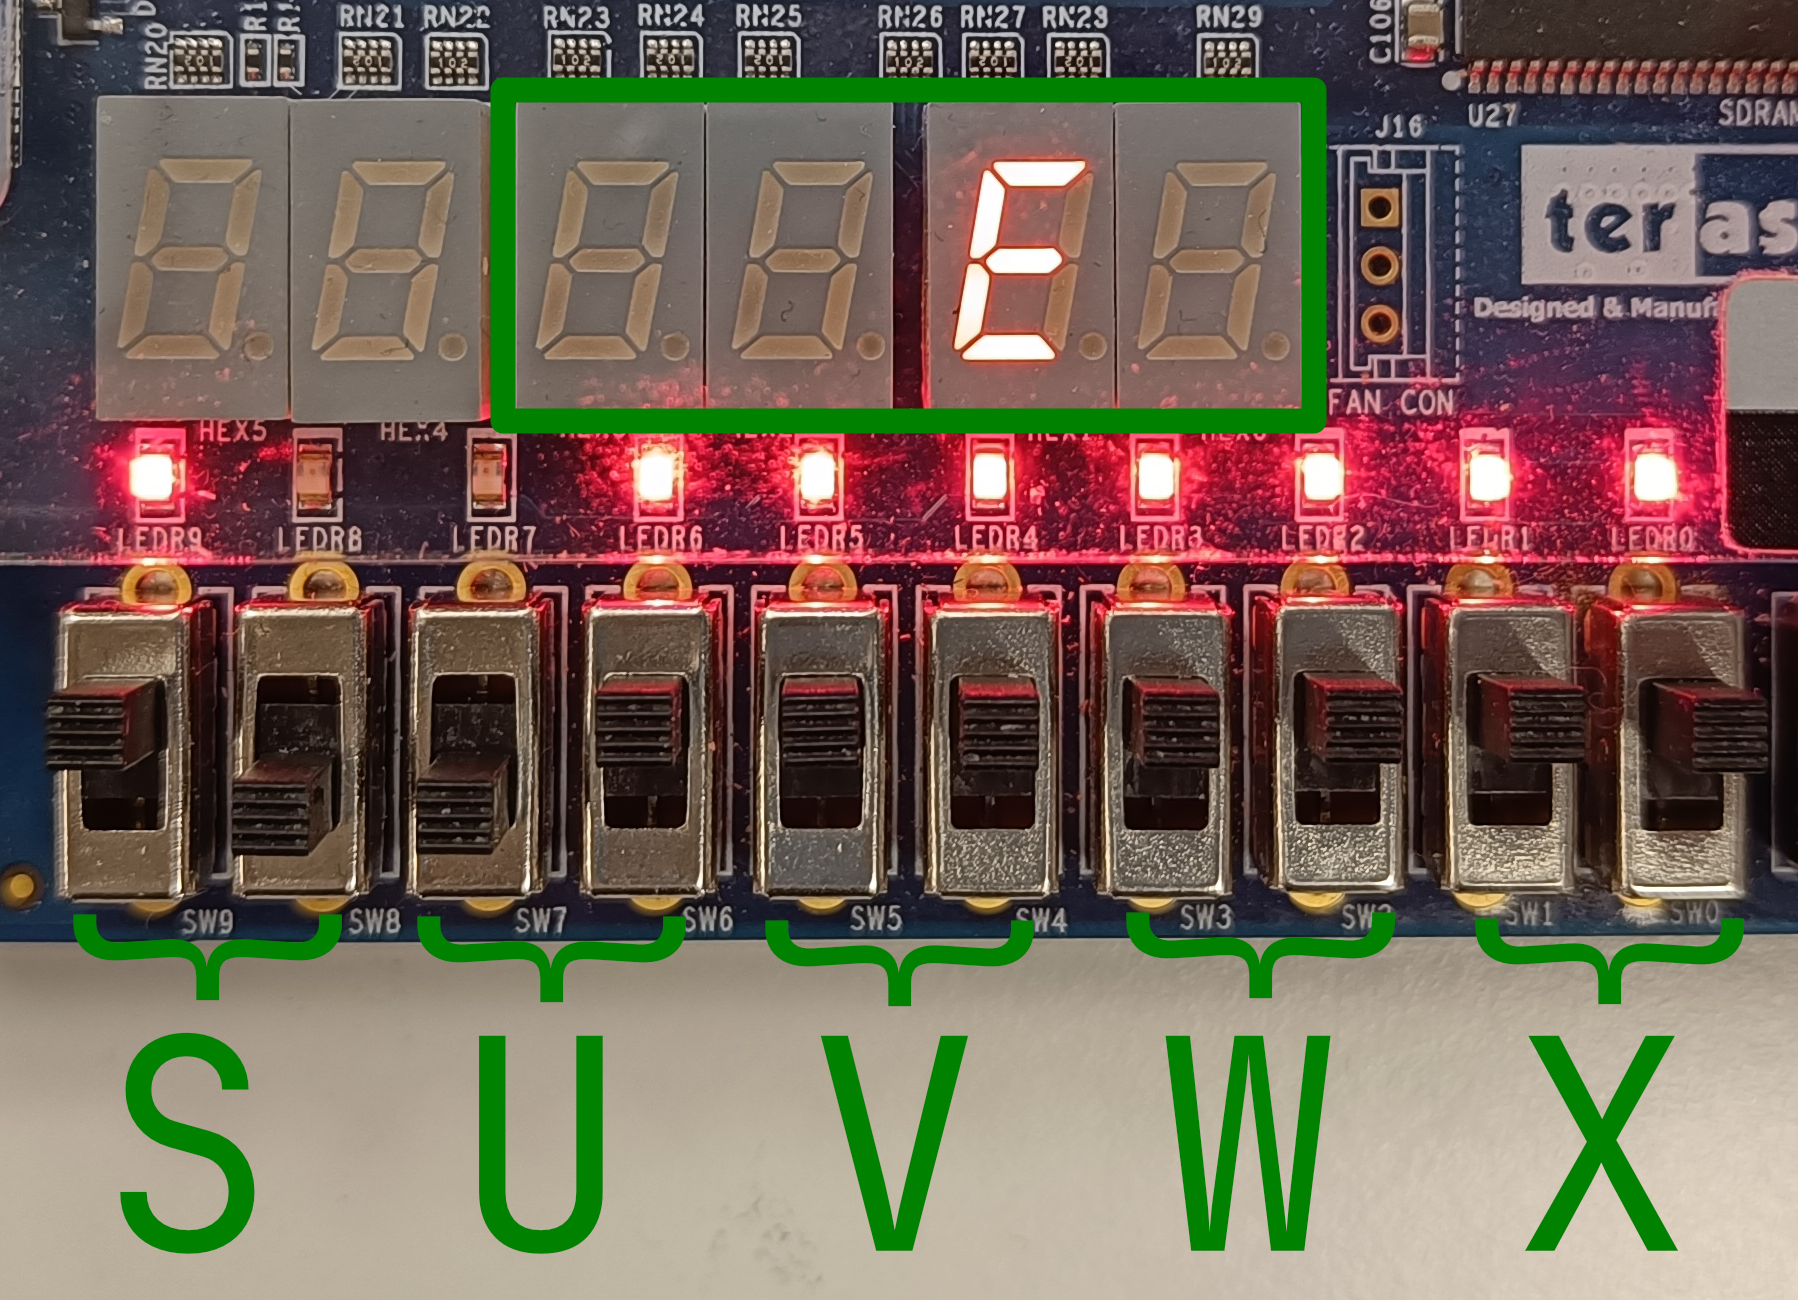
\includegraphics[width=1\textwidth]{Figures/Part5_E_10.png}
        \caption{E third at s = 10}
        \label{fig:T05epic3}
    \end{subfigure}
    \hfill
    \begin{subfigure}{0.45\textwidth}
        \centering
        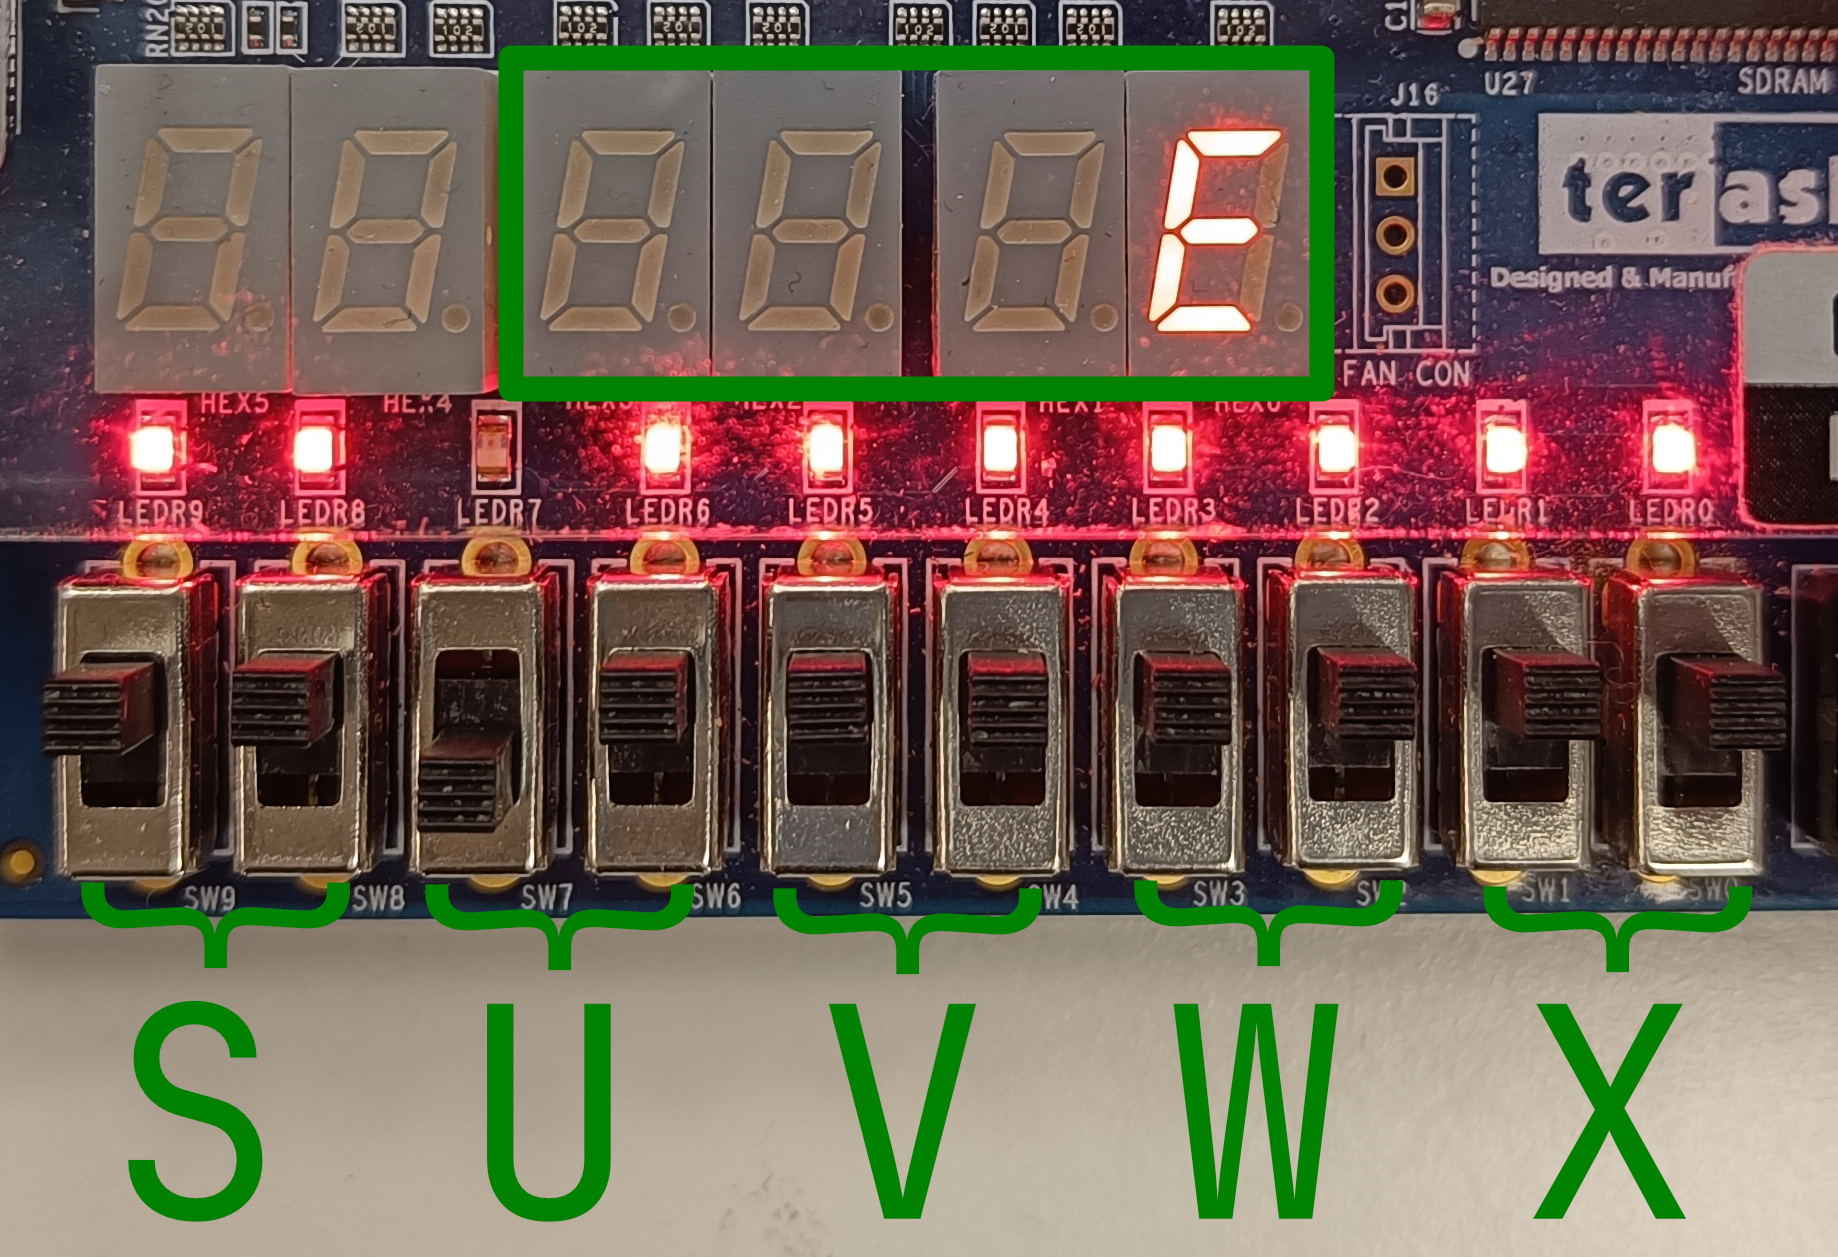
\includegraphics[width=1\textwidth]{Figures/Part5_E_11.png}
        \caption{E last at s = 11}
        \label{fig:T05epic4}
    \end{subfigure}
    \caption{Test results for "E   " input}
    \label{fig:T05epic}
\end{figure}
As you can see here as with the previous example it is very easy to see how the rotation. At U = 01 witch makes E and V, W and X = 11 wich makes the rest off, then only changing S between the photos clearly shows how the inputs are rotating along the multiplexer inputs.


\end{document}
